\documentclass[10pt]{article}
\usepackage[margin=22mm]{geometry}
\usepackage{amsmath,amssymb,graphicx,booktabs,array,enumitem,xcolor}
\usepackage[colorlinks=true,urlcolor=blue!55!black,linkcolor=blue!55!black]{hyperref}
\pagestyle{plain}
\setlength{\parindent}{0pt}\setlength{\parskip}{5pt}
\setlist{nosep,leftmargin=*}\setlength{\emergencystretch}{2em}
\newcommand{\um}{\,\mu\mathrm{m}}\newcommand{\E}{\mathbb{E}}
\graphicspath{{figures/}}
\newcommand{\FreeMeanError}{0.5801}
\newcommand{\MixedError}{0.9178}
\newcommand{\MixedErrorSE}{0.00008}
\newcommand{\MixedImprovement}{15.8}
\newcommand{\MixedTotal}{260,251}
\newcommand{\MixedRMSE}{4.86}
\newcommand{\MixedSeconds}{0.196}
\newcommand{\MixedAttempts}{305,019}
\newcommand{\MixedConverged}{0}
\newcommand{\MixedCapped}{0}
\newcommand{\TracerError}{0.9611}
\newcommand{\TracerErrorSE}{0.00006}
\newcommand{\TracerImprovement}{7.6}
\newcommand{\TracerTotal}{208,590}
\newcommand{\TracerRMSE}{5.09}
\newcommand{\TracerSeconds}{0.252}
\newcommand{\TracerAttempts}{231,459}
\newcommand{\TracerConverged}{1}
\newcommand{\TracerCapped}{0}
\newcommand{\PreviousError}{0.9056}
\newcommand{\PreviousErrorSE}{0.00008}
\newcommand{\PreviousImprovement}{18.0}
\newcommand{\PreviousTotal}{37,129}
\newcommand{\PreviousRMSE}{4.80}
\newcommand{\PreviousSeconds}{0.067}
\newcommand{\PreviousAttempts}{40,410}

\begin{document}
\begin{center}
{\LARGE A simple voxel SIS model of mouse pathology}\\[5pt]
{\large Model construction, measurement assumptions and a direct fit}\\[4pt]
\small 26 November 2026. Computational proof of concept; fits are conditional on the stated assumptions.
\end{center}

\section{What we have fitted}
We ask whether a small number of uniform spreading and clearance rates can reproduce the broad progression of mouse pathology on a tracer-derived spatial network. We use the finest prepared model, with 448,962 voxels of side $100\um$, and estimate its mean by simulating the count process directly. Anatomical regions are used to read out the simulations; they are not the simulation nodes.

The new fit removes the free observation amplitude. It treats modeled affected cells as immediately detectable and approximates the measurement by counting cell centers in a $6\um$ tissue slab. This is a deliberately simple measurement assumption, not a stereological correction. We also retain the earlier fit with a free scale as a comparison. We have not added a latent stage, a detection delay, region-specific rates or cell-type vulnerability.

The fixed-depth mixed model has relative RMS error \MixedError{}, versus \TracerError{} for tracer-only and \PreviousError{} for the earlier freely scaled mixed fit. A model predicting zero everywhere has error 1. The fixed-depth mixed fit reduces squared error by \MixedImprovement{}\% relative to that zero prediction. These are in-sample results, not evidence that the microscopic parameters have been identified.

\section{The stochastic model}
Voxel $i$ contains a fixed integer population $N_i$. Its state $I_i(t)\in\{0,\ldots,N_i\}$ is the number of affected cells. It is not a binary label for the entire voxel. The remaining $N_i-I_i$ cells are susceptible. An affected cell may clear its affected state and become susceptible again; this does not model cell death or replacement.

With sources in matrix rows and destinations in columns, define
\begin{align}
 I_i&\longrightarrow I_i+1
 &&\text{at rate }\lambda_i(I)=\left(1-\frac{I_i}{N_i}\right)
       \sum_j\left[\beta_T Q_{ji}+\beta_L L_{ji}\right]I_j,\label{eq:sis}\\
 I_i&\longrightarrow I_i-1
 &&\text{at rate }\mu_i(I)=\gamma I_i.\nonumber
\end{align}
Time is in months. The three uniform parameters $\beta_T,\beta_L,\gamma$ have units month$^{-1}$. $Q$ is the dimensionless, strength-preserving tracer contact matrix; $L$ is a dimensionless local contact matrix with row sums one. Thus $\beta_L$ is the local contact-attempt rate per affected cell, while the tracer attempt rate at source $j$ is $\beta_T\sum_i Q_{ji}$. An attempted contact succeeds only if its target cell is susceptible.

\textbf{What is exact?} Assume that all cells in a voxel obey the same contact rule, and that targets within a destination voxel are chosen uniformly. Summing this cell process gives Eq.~\ref{eq:sis} exactly. The simulator therefore needs counts rather than tens of millions of individual cell labels. This is an exact reduction of the assumed block-homogeneous contact model. It is not an exact reconstruction of real neuron-to-neuron wiring.

The mean is estimated by $\widehat{\E I_i(t)}=R^{-1}\sum_{r=1}^{R}I_i^{(r)}(t)$, using independent realizations. No mean-field factorization or deterministic ODE is used in fitting. In particular, the nonlinear term in Eq.~\ref{eq:sis} is evaluated on each stochastic state, not on the ensemble mean.

\newpage
\section{Data used to construct the model}
\subsection{The grid and tracer contacts}
The grid comes from the Allen annotation and the domain of the Knox et al. voxel connectivity model [1,2]. Cubes have volume $v=10^6\um^3=0.001\mathrm{\,mm}^3$. The annotation grid is $132\times80\times114$; the prepared mask contains 448,962 cubes. Atlas labels provide anatomical names and measurement windows. They do not impose homogeneous regional dynamics.

The published tracer model uses 428 experiments and infers source connectivity by spatial interpolation within major anatomical divisions [1]. We use its released nonnegative factors, written $W=UV$, where $W_{ji}$ is a source-to-target projection weight. These are tracer-derived relative weights, not measured synapse counts or probabilities for every voxel pair. The $100\um$ spacing is a model grid, not independent experimental resolution. We preserve the prepared factors; no extra threshold is applied in this fit.

The release supplies right-hemisphere sources and bilateral targets. The prepared reference supplies left sources by reflecting both source and target coordinates. At mask boundaries, the nearest supported voxel is used. The largest recorded displacement is $223.6\um$; 10,640 source lookups and 25,010 target reflections are non-exact. Bilateral symmetry is a model assumption.

Let $D=\mathrm{diag}(N_1,\ldots,N_n)$ and fix one global normalization
\begin{equation}
 c=\frac{\sum_jN_j\sum_iW_{ji}}{\sum_jN_j}
   =24.381317861482305,\qquad
 Q=D^{-1}(W/c)^\mathsf{T}D.\label{eq:q}
\end{equation}
We use the reverse contact direction as a fixed hypothesis. It is not selected in this fit. The population factors matter: the forward per-cell pair weight is $W_{ji}/(cN_i)$. Reversing those cell-level edges gives $Q_{ji}=N_iW_{ij}/(cN_j)$, rather than simply transposing the voxel matrix. The population-weighted mean outgoing strength is one; individual rows need not sum to one. Thus we retain variation in tracer-derived contact strength. Sparse factors allow sampling without constructing a dense $n\times n$ matrix.

\subsection{Population counts from MERFISH}
We use registered neuronal detections from Allen reference animal 638850 [3]. Of 2,126,285 neuronal detections in the prepared data, 1,973,822 fall inside the model mask. To estimate a volumetric population, we assume $10\um$ sampled sections at $200\um$ intervals and multiply counts by 20. This assumes representative sampling and ignores detection bias. It is a density prior from one reference animal, not a census of the pathology mice.

To fill the gaps between sampled sections, each retained detection contributes a Gaussian density with $\sigma_N=200\um$, truncated at four standard deviations and normalized within the modeled mask. The implementation uses a separable discrete Gaussian. We round to integers, impose at least one cell per modeled voxel and distribute the remaining rounding residuals to conserve the total. The resulting population is 39,476,440; the median voxel has 83 cells and the maximum has 354. The frozen preparation used quantized registered coordinates. Its center-versus-edge coordinate convention remains a registration uncertainty; this fit does not shift those arrays.

\subsection{An additional local channel}
For voxel-center distance $d_{ji}$, the retained local rule is
\begin{equation}
 L_{ji}=\frac{N_i\exp[-d_{ji}^2/(2\sigma_L^2)]\mathbf{1}_{d_{ji}\leq r_L}}
 {\sum_kN_k\exp[-d_{jk}^2/(2\sigma_L^2)]\mathbf{1}_{d_{jk}\leq r_L}},
 \qquad \sigma_L=200\um,\quad r_L=600\um.\label{eq:local}
\end{equation}
The sum includes $i=j$, so within-voxel contacts occur. Targets outside the model mask are excluded. Row normalization fixes the total local attempt rate, even near boundaries or in low-density tissue. This is a retained assumption, not a measured short-range connectome. The tracer model already contains some near-source signal, so this channel is an additional hypothesis and may overlap it. The tracer-only control sets $\beta_L=0$.

\newpage
\section{Initial condition and simulation}
The frozen initial state has 1,000 affected cells in 108 voxels near the right caudoputamen. The provisional center is $(5.55,3.25,7.95)$ mm in the prepared AP/DV/ML atlas convention. The initial allocation is proportional to $N_i\exp[-d_i^2/(2(150\um)^2)]$ inside a $300\um$ radius, with integer rounding preserving 1,000. The center was chosen near the dorsal quarter of the right caudoputamen. It is not a registered experimental injection location, and the 1,000-cell burden is not an experimentally estimated count. Both are fixed here, so the fitted rates are conditional on them.

One equivalent exact event algorithm is:
\begin{enumerate}
\item Form tracer-attempt rate $H_T=\beta_T\sum_j I_j q_j$, with $q_j=\sum_iQ_{ji}$, local-attempt rate $H_L=\beta_L\sum_jI_j$, and recovery rate $H_R=\gamma\sum_jI_j$.
\item Advance by an exponential waiting time with rate $H_T+H_L+H_R$ and choose the channel in proportion to these rates.
\item For tracer contact, choose source $j$ proportional to $I_jq_j$ and destination $i$ with probability $Q_{ji}/q_j$. For local contact, choose source proportional to $I_j$ and destination with probability $L_{ji}$. Accept the birth with probability $1-I_i/N_i$; otherwise it is a null event.
\item For recovery, choose $i$ proportional to $I_i$ and decrease its count by one. Repeat, recording the state at the requested observation times.
\end{enumerate}
The implemented sampler uses sparse-factor sampling, local rejection bounds and an equivalent susceptible-target proposal when useful. These accelerate the same generator. They do not introduce a time step or a closure. An attempt-limit violation raises an error; an incomplete trajectory is never treated as a complete simulation. Synthetic master-equation tests and unchanged seeded reference trajectories check the implementation.

\section{Pathology data used for fitting}
The target is the published regional density of inclusion-bearing cell-body profiles, in profiles/mm$^2$ of tissue section, from the study and analysis repository in [4,5]. It is distinct from total pathology area percentage, neuritic pathology, raw fluorescence and a 3D cell count.

We retain 18,292 mouse/window/time records from 55 mice at eight terminal timepoints:
\begin{center}
\begin{tabular}{lrrrrrrrr}\toprule
Months & .1 & .2 & .3 & .5 & 1 & 3 & 6 & 9\\
Mice & 4 & 4 & 4 & 8 & 8 & 12 & 8 & 7\\\bottomrule
\end{tabular}
\end{center}
These are different mice at different times, not repeated measurements of the same animals. Reported anatomical IDs and their descendants define 648 distinct hemisphere-specific windows. Within each mouse, the most specific available nonoverlapping windows are retained, avoiding double counting tissue. This gives 3,553 observed window/time combinations. Measured zeros are retained; missing measurements are omitted.

The combined later-time CSV labels the density column ``log10'', but its stored values include zero and reach 218.84. We preserve the numeric values as density, without exponentiation, consistently with the earlier density columns and the intended processing formula. The exact export checkpoint still needs confirmation. The NutilToUsable code [6] describes a ratio of mean object count to mean region area; one branch has a conflicting later assignment. Thus that source supports the intended measurement, but does not establish bit-for-bit provenance of the exported density column.

The project also contains 904 registered section/hemisphere JSON exports covering 55 mice and about 23 million positive coordinates, plus a raw-image pilot for mouse WT11. They are not used in these fits. Positive coordinates alone do not identify measured tissue with zero pathology, and their point semantics need confirmation before treating them as cell counts. The available atlas footprints are not verified tissue masks.

\newpage
\section{An explicit, minimal observation model}
\subsection{The physical measurement we would like to reproduce}
Let $C_{mgs}$ be the positive-object count in mouse $m$, region $g$, section $s$, and $A_{mgs}$ its sampled area in mm$^2$. If the same sections contribute to both summaries, the density is
\begin{equation}
 y_{mg}=\frac{\sum_s C_{mgs}}{\sum_s A_{mgs}}.
\end{equation}
For ideal point-like cells, let $V_{mgsi}$ be the intersection volume in $\um^3$ between sampled tissue and voxel $i$. Uniform positions within voxels would give
\begin{equation}
 \widehat C_{mgs}=\sum_i\frac{V_{mgsi}}{v}\E I_i(t_m),\qquad
 \widehat y_{mg}=\frac{\sum_s\widehat C_{mgs}}{\sum_s A_{mgs}}.\label{eq:section}
\end{equation}
This is a direct count-and-geometry measurement model. It does not require an arbitrary regional amplitude. However, registered tissue masks and a verified raw count/area checkpoint are not available as a complete fitted bundle here, so Eq.~\ref{eq:section} is not the implemented section-level fit.

\subsection{The approximation actually fitted}
We assume the sampled sections represent the whole modeled anatomical window and use the $6\um$ section thickness reported in the study methods [4, PDF p.~18]. The methods describe nuclear-based cell detection, a positive-cell classifier and Nutil object/area summaries [4, p.~19]. Define
\begin{equation}
 O_{gi}=\frac{\mathbf{1}_{i\in g}}{V_g},\qquad V_g=v\,|g|,
 \qquad \rho_g(t)=\sum_i O_{gi}\E I_i(t).
\end{equation}
$\rho_g$ has units cells/$\um^3$. The new prediction is
\begin{equation}
 \boxed{\widehat y_{mg}=10^6 h\,\rho_g(t_m),\qquad h=6\um\ \text{fixed}.}\label{eq:obs}
\end{equation}
The $10^6$ converts area from $\um^2$ to mm$^2$. The number of sections does not multiply $h$: it cancels between summed counts and summed areas. The denominator is the full window's modeled volume, not the voxel population; MERFISH affects the dynamics through $N_i$, while the observation is affected-cell density.

Equation~\ref{eq:obs} assumes immediate detectability, perfect detection, point-like cell centers and representative regional sampling; it ignores tissue shrinkage and registration volume changes. In reality, the experimental count is a profile count. For the idealized case of counting every intersected object, detection fraction $p$ and mean object extent $\bar d_\perp$ normal to the section would instead give an effective depth $p(h+\bar d_\perp)$. Neither this geometry nor detection is calibrated here. Setting the depth to $h$ is therefore a transparent first approximation, not a claim that physical thickness alone solves the measurement problem.

For comparison, the earlier fit used $\widehat y=a10^6\rho_g$ with one common nonnegative fitted $a$. At fixed predicted densities $x_r=10^6\rho_{g(r)}(t_r)$, its best scale is
\begin{equation}
 a^*=\max\left(0,\frac{\sum_r w_r x_r y_r}{\sum_r w_r x_r^2}\right).
\end{equation}
Its value, $43.79\um$, is an empirical conversion, not a measured section thickness. It may compensate for initial burden, profile geometry, sampling or model mismatch. We retain that result as a benchmark, not as a biological estimate of capture depth.

\newpage
\section{Fitting method and comparison}
The new fits estimate $\theta=(\beta_T,\beta_L,\gamma)$ for mixed contacts and $(\beta_T,\gamma)$ for tracer-only. All rates are constrained to $[0,1]$ month$^{-1}$; $\beta_L=0$ is fixed in tracer-only. Population, connectivity direction and normalization, initial condition, local length scale and observation windows are fixed. No coarser network is used to evaluate candidates.

For record $r$ from mouse $m$ at time $t$, we minimize
\begin{equation}
 J(\theta)=\frac{\sum_r w_r\big[\widehat y_r(\theta)-y_r\big]^2}
 {\sum_r w_r y_r^2},\qquad
 w_r=\frac{A_r}{\sum_{r'\in m} A_{r'}}\frac{1}{M_t}\frac{1}{8}.\label{eq:loss}
\end{equation}
$A_r$ is the supplied regional-area summary and $M_t$ is the number of mice at time $t$. These area summaries are used as weighting proxies, not asserted to be reconstructed total sampled areas. Each mouse has equal total weight within its timepoint and each timepoint has equal total weight. Large absolute density errors still contribute more than small ones. We fit individual mouse records, rather than first fitting a timepoint-average map. The reported relative RMS error is $\sqrt J$.

We use bounded Nelder--Mead with two starts per model. Each objective evaluation uses 32 complete CTMC realizations with a common seed set. The budget is 80 evaluations per start, with parameter tolerance 0.002 and objective tolerance $10^{-5}$. Each finalist is reevaluated with 256 fresh realizations. The selected candidate is evaluated with another 512 realizations for the reported figures and errors. Fresh simulations test Monte Carlo stability; all mouse data remain in the fit. This is not held-out biological validation and is not a guaranteed global optimum. Search convergence and capped evaluations are saved alongside each candidate.

The earlier freely scaled fit used its previously saved, separate search: a 22-candidate screen, three searches with 64 paths per evaluation, 512-path finalist comparisons and a 1,024-path final ensemble. It used a different search parameterization and rate bounds. Its row below is a historical benchmark, not an equal-budget test of algorithms.

\begin{center}\small
\begin{tabular}{lrrrrrr}\toprule
Model & $\beta_T$ & $\beta_L$ & $\gamma$ & Depth $a$ & Rel. RMS & $R_w^2$\\
 & \multicolumn{3}{c}{month$^{-1}$} & $\um$ & &\\\midrule
Mixed, fixed depth & 0.1232 & 0.4749 & 0.0035 & 6.00 & 0.9178 & 0.126 \\
Tracer, fixed depth & 0.5047 & 0.0000 & 0.0000 & 6.00 & 0.9611 & 0.042 \\
Mixed, fitted scale & 0.1477 & 0.2137 & 0.0012 & 43.79 & 0.9056 & 0.149 \\
\bottomrule\end{tabular}

\end{center}
Here $R_w^2=1-\sum_r w_r(\widehat y_r-y_r)^2/\sum_r w_r(y_r-\bar y_w)^2$, with $\bar y_w=\sum_r w_r y_r$. It compares with a weighted constant prediction, whereas relative RMS compares with zero. Monte Carlo SEs of relative RMS are \MixedErrorSE{} (mixed) and \TracerErrorSE{} (tracer-only). These quantify numerical uncertainty at fixed parameters, not uncertainty in fitted rates or biological variability.

Of the two starts per family, \MixedConverged{} mixed and \TracerConverged{} tracer-only searches satisfied the convergence criteria; the others exhausted their evaluation budgets. There were \MixedCapped{} and \TracerCapped{} capped evaluations, respectively. No capped path contributed to a reported objective or final mean.

The selected tracer-only fit has $\gamma=0$, the no-recovery (SI) boundary. The mixed fit also uses little clearance. These conditional fits do not establish that biological clearance is absent, and they do not reproduce the strong peaks and declines in several measured regions.

As a descriptive comparison, an independently fitted mean for every observed window/time combination reaches relative RMS \FreeMeanError{}. This uses many more parameters and all the same data; it is neither a biological noise floor nor a validated prediction. It shows how much room remains beyond the uniform SIS fit even after allowing for variation between mice in the same window/time group.

\newpage
\section{What the fit looks like}
The mixed fixed-depth model predicts \MixedTotal{} affected cells at nine months; tracer-only predicts \TracerTotal{}. The historical freely scaled model predicts \PreviousTotal{}. The mixed model's inferred burden changes roughly sevenfold when the measurement conversion is fixed. These are latent modeled totals, not counts measured across entire pathology brains. Their dependence on the observation conversion illustrates why a good-looking fit alone cannot identify absolute biological burden.

\begin{center}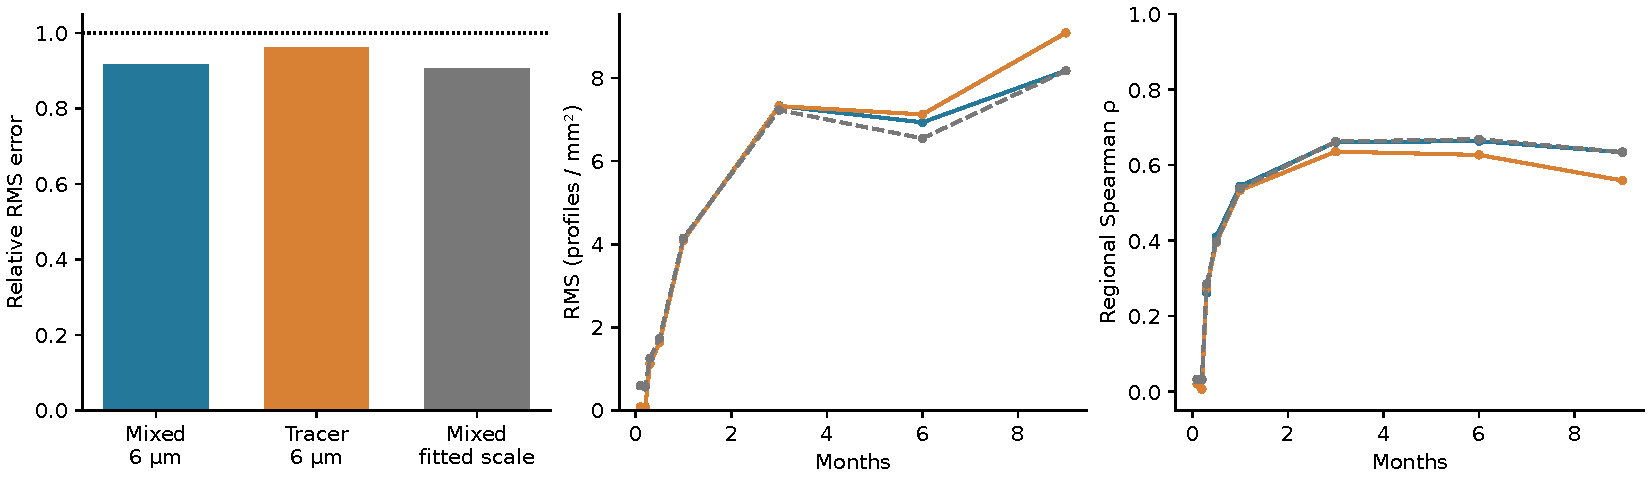
\includegraphics[width=\linewidth]{fit_comparison.pdf}\end{center}
\small\textbf{Figure 1.} Fit errors and regional pattern agreement. The dotted line is zero prediction. Regional correlations use equal-mouse means for each reported label at each time. Colors match subsequent trajectory plots. Correlation can be reasonable while absolute error remains large.\normalsize

\begin{center}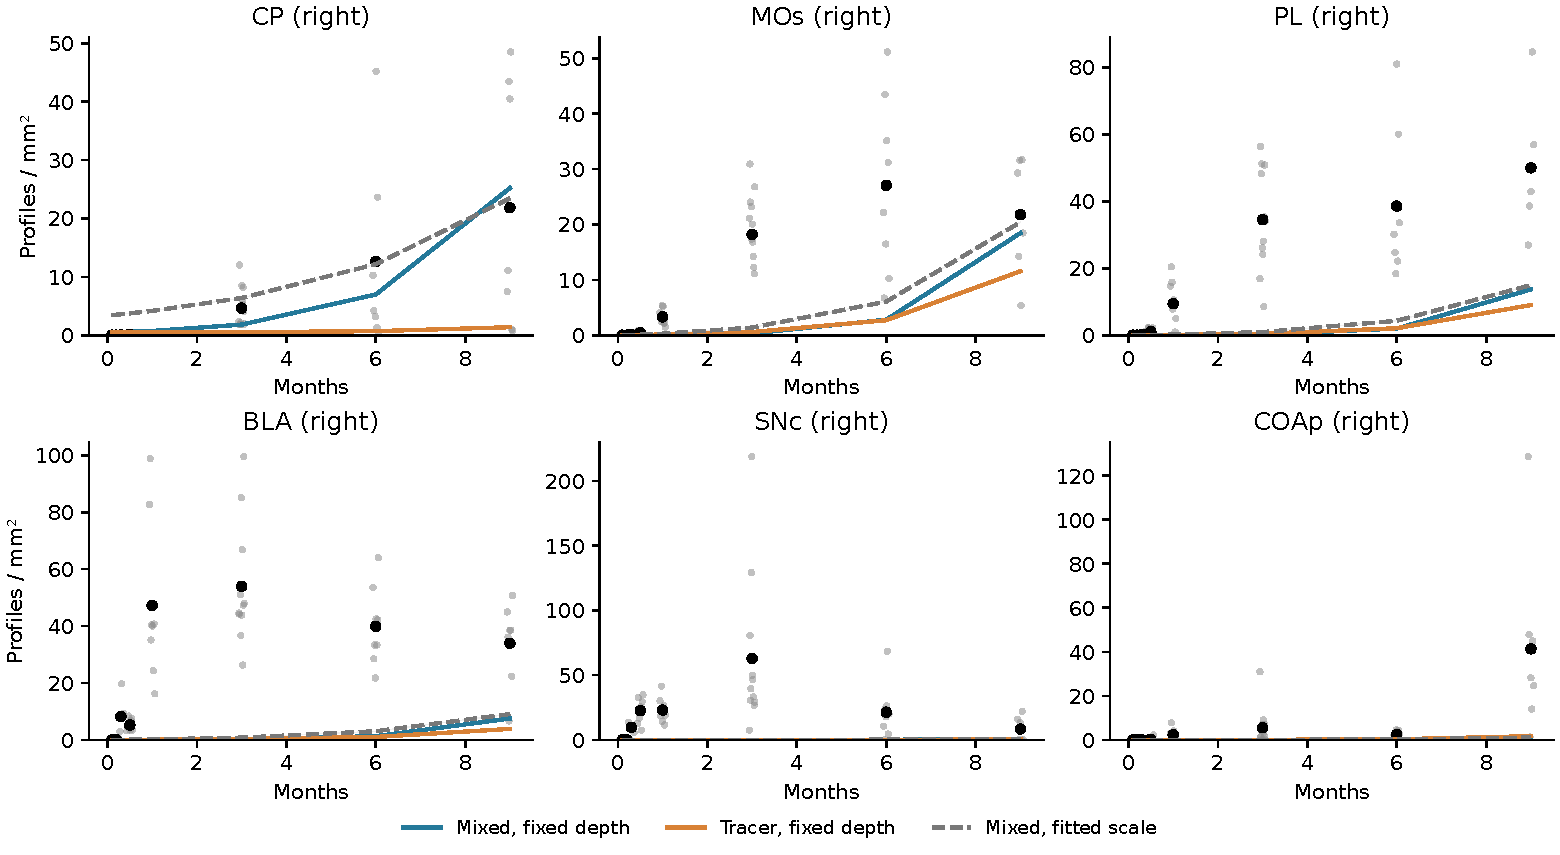
\includegraphics[width=\linewidth]{regional_trajectories.pdf}\end{center}
\small\textbf{Figure 2.} Six illustrative right-hemisphere regions. Gray dots are individual mice; black dots are their means. Lines are model ensemble means, mapped to the same reported windows. Narrow bands show $\pm1.96$ Monte Carlo SE, not between-mouse variation or parameter confidence intervals. Missing label/time combinations are not set to zero. The connecting lines guide the eye between evaluated times. CP: caudoputamen; MOs: secondary motor cortex; PL: prelimbic cortex; BLA: basolateral amygdala; SNc: substantia nigra pars compacta; COAp: posterior cortical amygdalar area.\normalsize

\newpage
The fixed-depth mixed fit is much too late in several regions. At three months, right SNc has a measured mean of 62.85 profiles/mm$^2$ but a predicted mean of about 0.01. At one month, right BLA is 47.27 in the data and about 0.02 in the model. By nine months, right CP is closer (21.84 measured, 25.21 predicted). Thus matching some late regional amplitudes does not recover the observed sequence of involvement.

The following slice figures apply the same regional averaging to model and data, then paint the regional means on the atlas. These are not raw histology images or independent voxel measurements. Each pair places the model directly above the data. The scale is shared across times and between the mixed and tracer-only figures. Gray means no regional measurement; it does not mean a measured zero. Fine-scale simulated maps remain available in the saved ensembles, but there is no fine-scale data fit in this report.

\begin{center}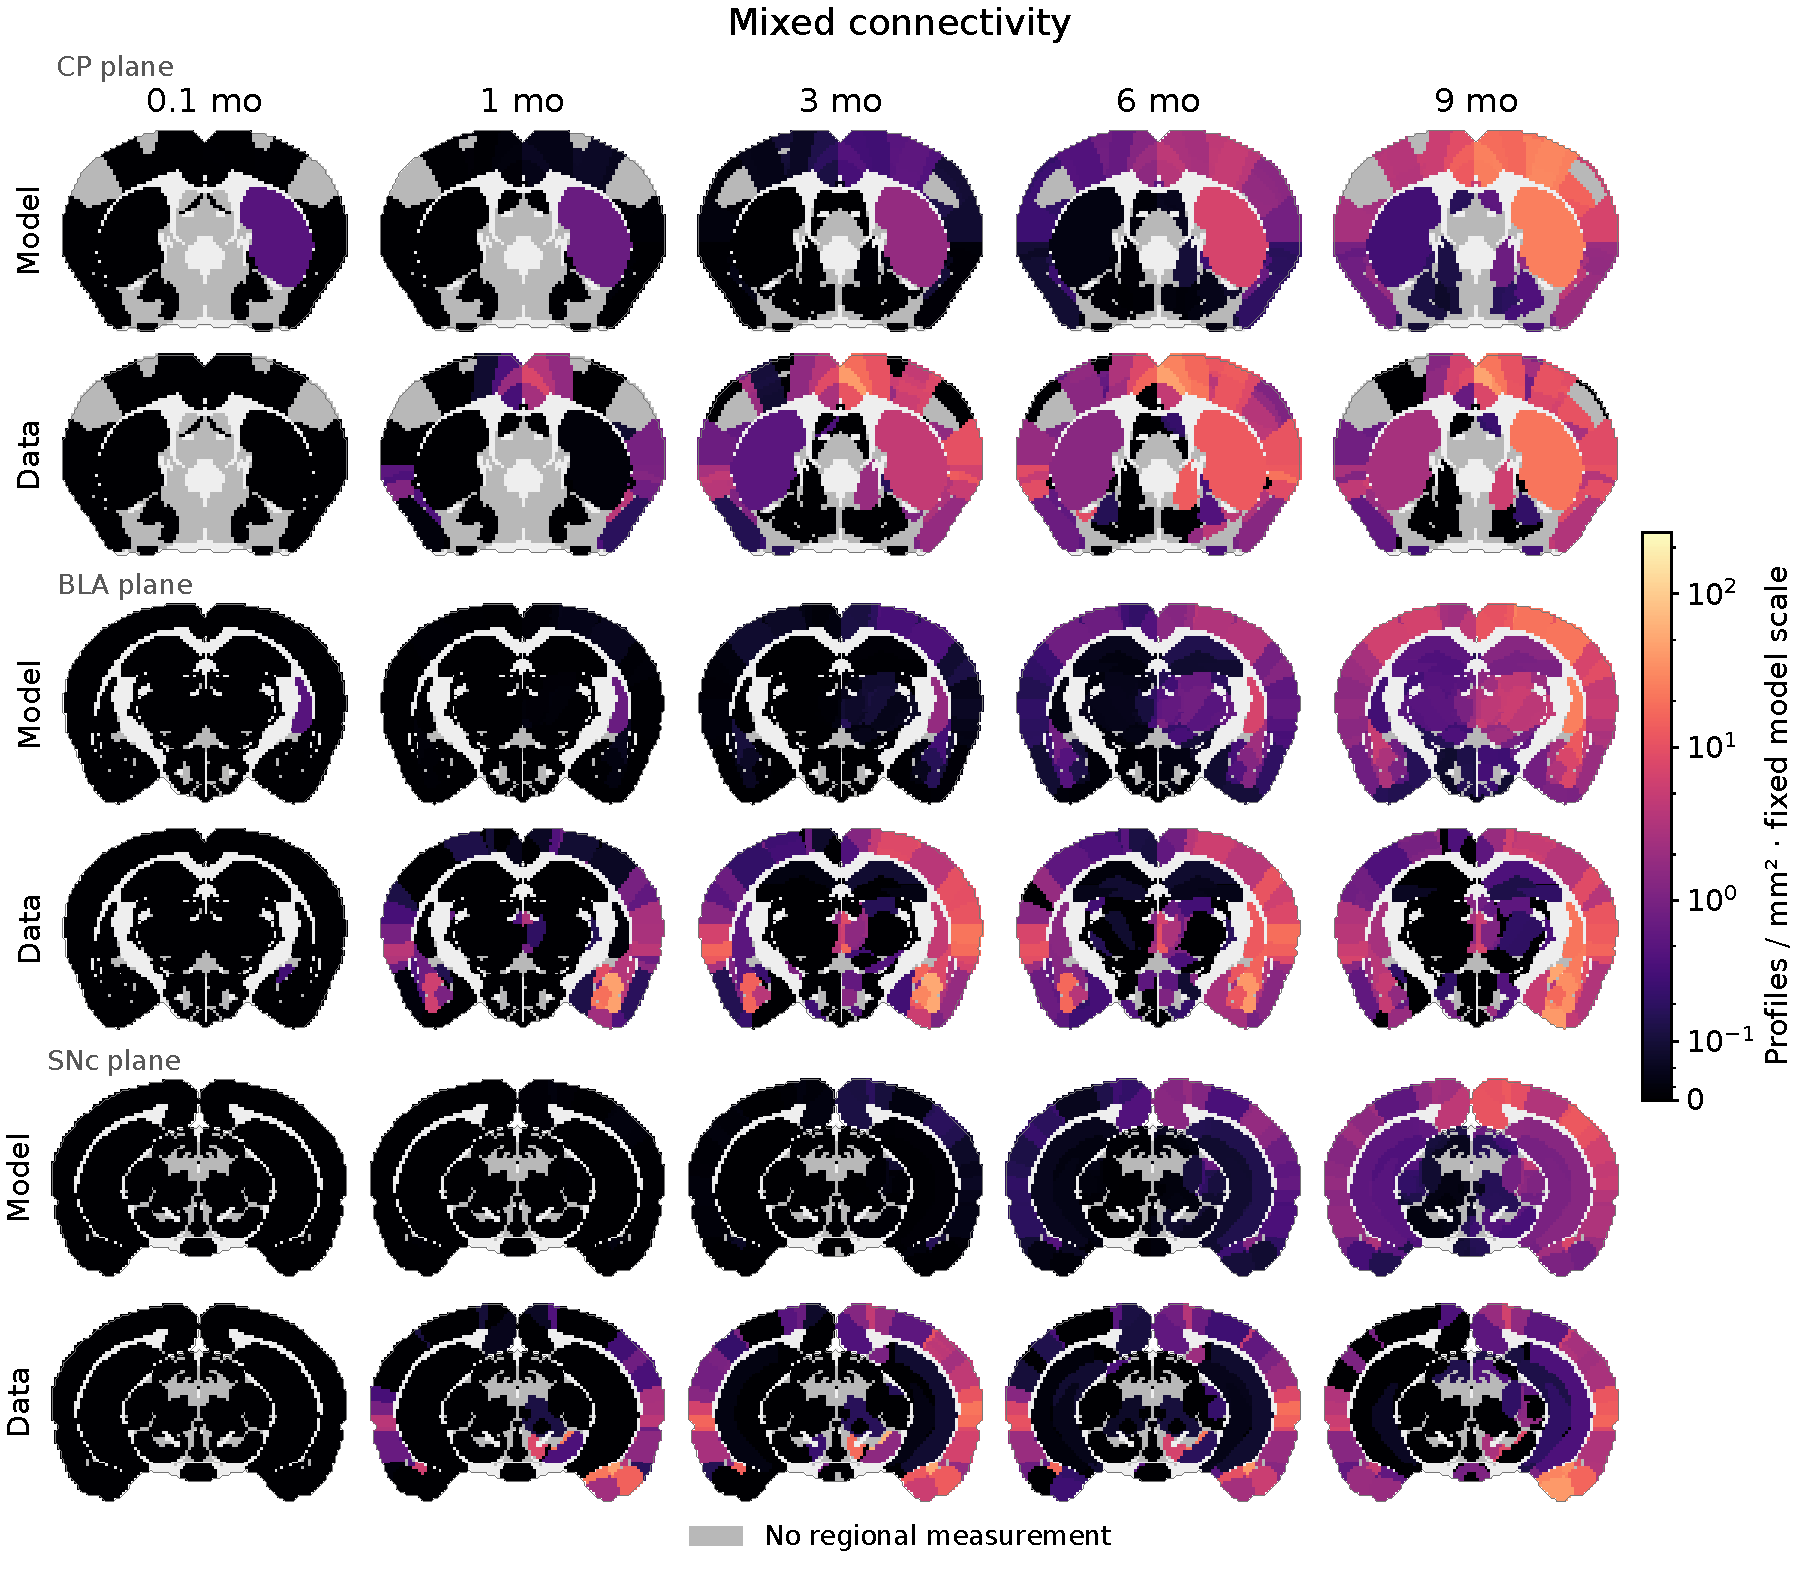
\includegraphics[width=\linewidth,height=.86\textheight,keepaspectratio]{mixed_regional_slices.pdf}\end{center}
\small\textbf{Figure 3.} Mixed connectivity, fixed $6\um$ readout. Rows show coronal planes at AP indices 55, 72 and 83 (approximately 5.55, 7.25 and 8.35 mm in the prepared center convention). Model and data use matching regional windows. The nonlinear color scale is fixed across all panels; it expands small values without changing their numerical predictions.\normalsize

\newpage
\begin{center}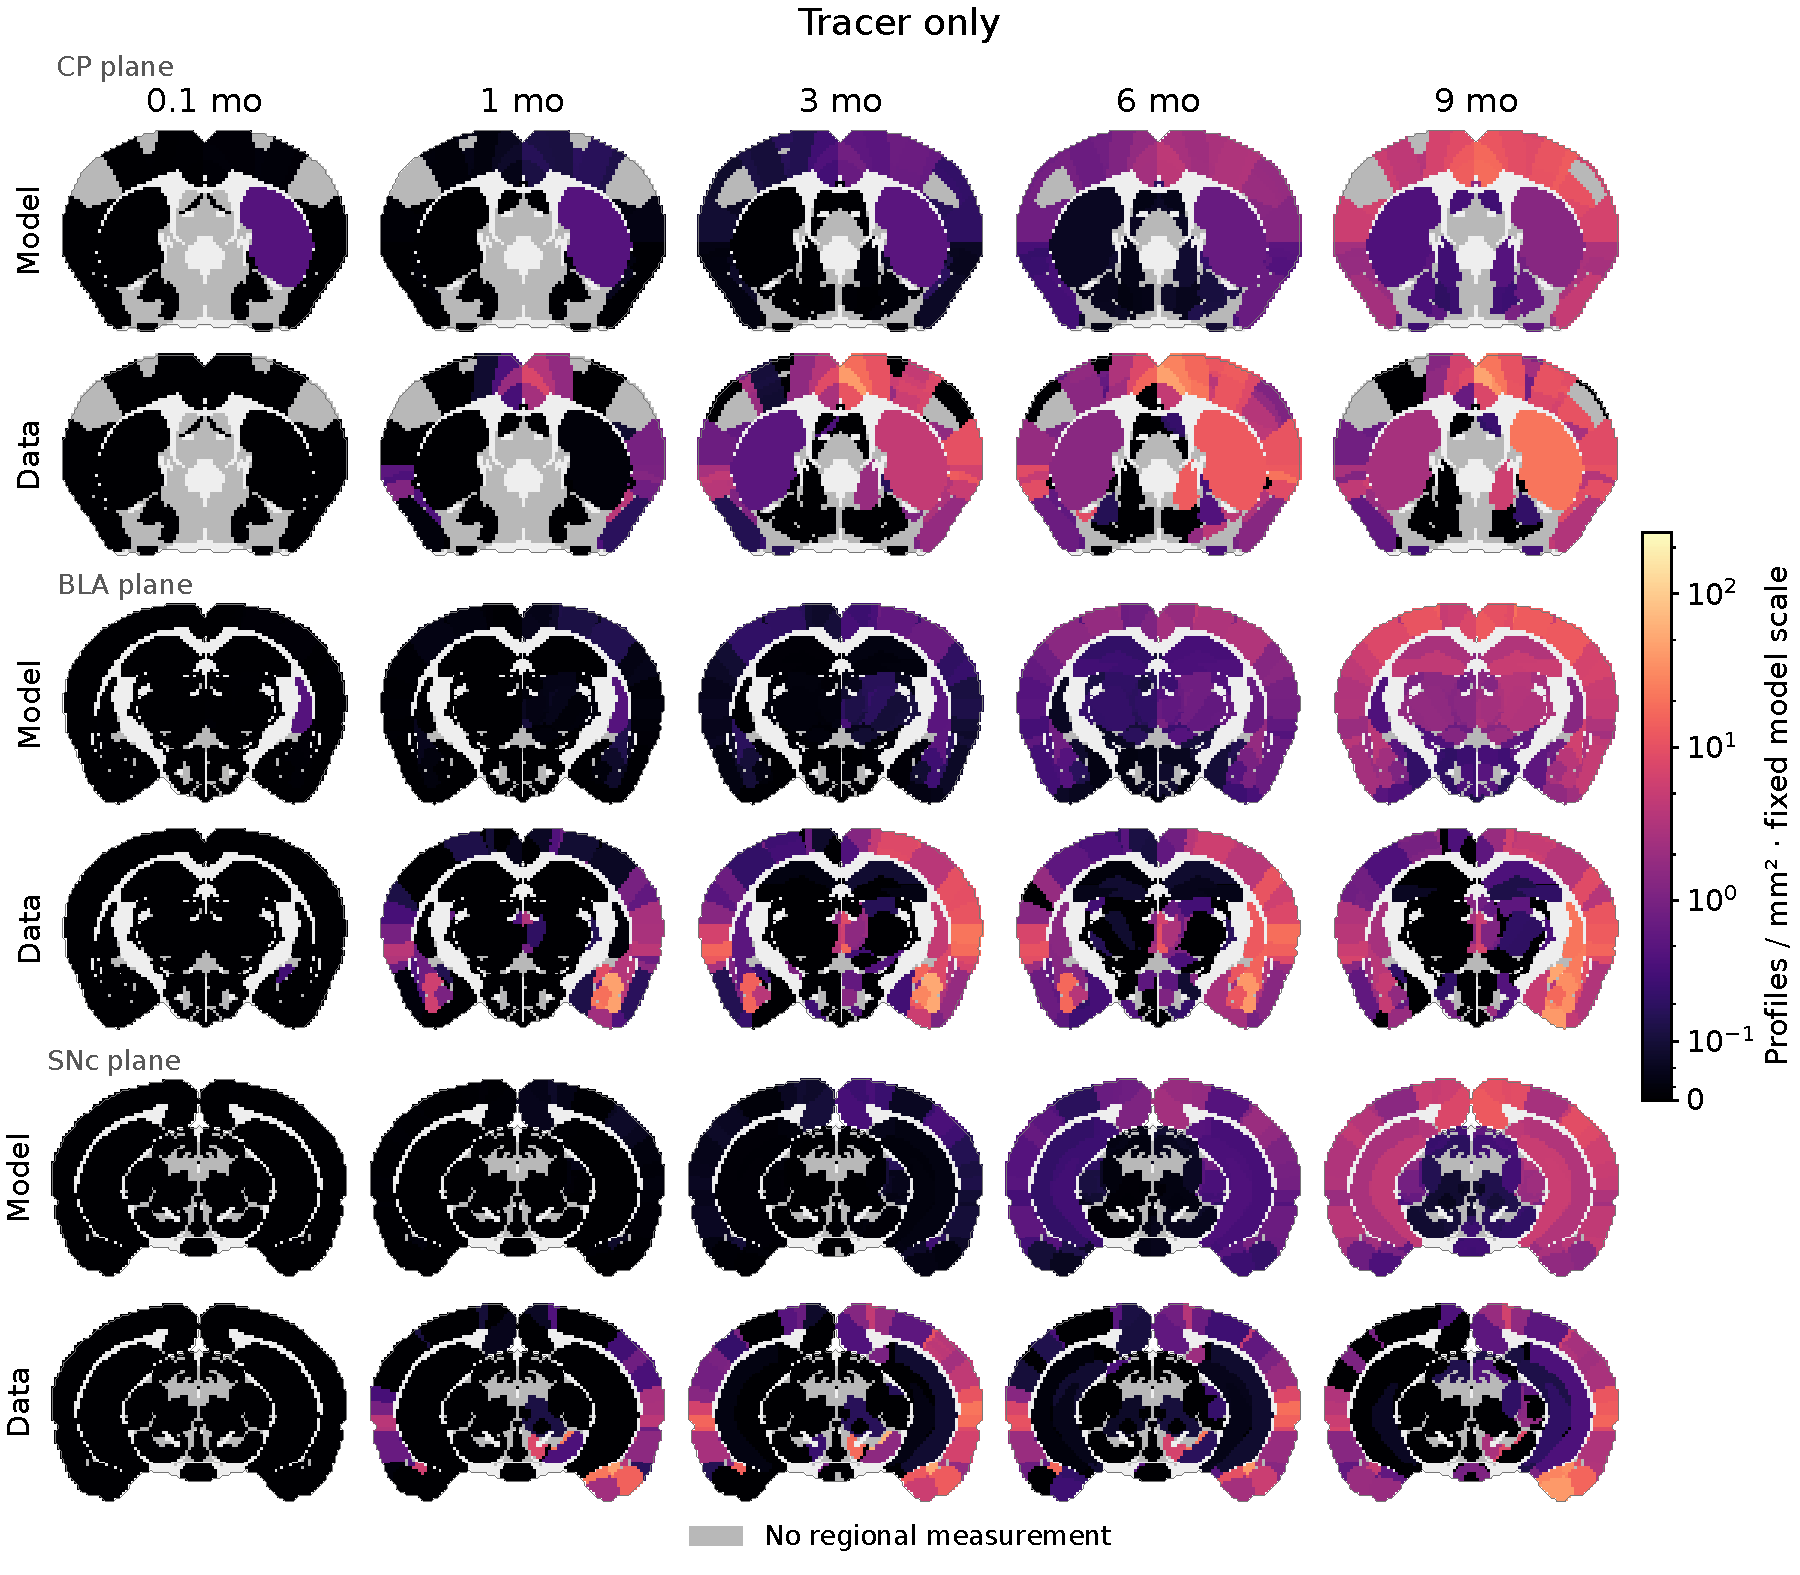
\includegraphics[width=\linewidth,height=.86\textheight,keepaspectratio]{tracer_only_regional_slices.pdf}\end{center}
\small\textbf{Figure 4.} Tracer-only connectivity, otherwise the same measurement and display rules as Figure 3. This tests whether adding the local channel improves this conditional fit. It does not establish that local biological transmission is absent or present: the tracer model already contains near-source signal and other model assumptions remain uncertain.\normalsize

\newpage
\section{What this establishes, and what it does not}
We now have a concrete path from a specified cell-count process to the measured density, with only two or three free dynamical parameters in the new fit. The physical-depth approximation makes the amplitude assumption explicit. It also makes its shortcomings visible. We have not established a quantitatively true biological model, reconstructed a microscopic connectome, inferred neuronal susceptibility, or fitted the raw section images.

The main uncertainties are:
\begin{itemize}
\item \textbf{Measurements:} cell-body profiles are not a stereological cell census; the $6\um$ point-center approximation omits object extent and detection. Full-region averages substitute for actual sampled tissue. The density-column export needs confirmation.
\item \textbf{Initial condition:} seed position and affected-cell burden are provisional. In dilute regimes, a change in initial burden can resemble a change in measurement amplitude. The fitted rates are conditional on the frozen seed.
\item \textbf{Contacts and populations:} tracer interpolation, reflection, direction reversal and local normalization are assumptions. MERFISH provides a smoothed reference-animal prior. The reference's coordinate convention needs a dedicated registration check.
\item \textbf{Dynamics and fitting:} immediate SIS readout treats all affected cells alike. Clearance is not neuronal death. Fits use all available mouse records and finite simulation/search budgets; no parameter-identifiability or predictive-validation claim follows from them.
\end{itemize}

The next useful step is a measurement check, not an immediate increase in model complexity. For one well-registered mouse, recover matched positive-object counts, section tissue areas and the counting definition; reproduce its exported regional density. Then use the same tissue masks in Eq.~\ref{eq:section}. If that agrees, apply it to more mice. Keep the same uniform SIS dynamics initially. A profile-size correction can be added as a measured quantity if needed, instead of introducing an unexplained global amplitude or biological delay.

For later resolution tests, first freeze this reference model, its microscopic parameters and its observation operator. Compare coarser simulations through the same measurement map. Refitting parameters at every resolution would mix coarse-graining error with parameter compensation; that is a different question.

\section{Reproduction and implementation}
The public code is \href{https://github.com/gretarsson/pixel-sis}{github.com/gretarsson/pixel-sis}. It separates the CTMC kernels, model loader, observation operator, fitter and plots. The numerical environment is Python 3.9.6, NumPy 2.0.2, SciPy 1.13.1, Numba 0.60.0 and Matplotlib 3.9.4. All new fits run on one numerical CPU thread. The new searches and final ensembles took about 43.5 minutes, excluding model loading. Median final-path times are \MixedSeconds{} s (mixed) and \TracerSeconds{} s (tracer-only), excluding compilation; their largest attempt counts are \MixedAttempts{} and \TracerAttempts{}, below the 2,000,000 cap.

The public repository contains code and input schemas, not the complete prepared mouse bundle or shared coordinate archives. Consequently, the synthetic example runs immediately after installation; reproducing the mouse fit additionally requires the prepared files listed in Appendix A. This report does not claim raw-data-to-fit reproduction from the public repository alone.

\small\begin{verbatim}
export OPENBLAS_NUM_THREADS=1 OMP_NUM_THREADS=1
export VECLIB_MAXIMUM_THREADS=1
python examples/run_section_fits.py \
  --data /path/to/tracer_sis/data --out results/section-fit
python examples/analyze_section_fits.py \
  --data /path/to/tracer_sis/data --fits results/section-fit \
  --previous /path/to/homogeneous_100um_direct --out report-figures
pytest -q
PIXEL_SIS_REFERENCE_DATA=/path/to/tracer_sis/data pytest -q -m reference
\end{verbatim}\normalsize

\newpage
\appendix
\small\setlength{\parskip}{3pt}
\section{Exact run settings and prepared inputs}
The new mixed starts are $(.25,.35,.05)$ and $(.35,.15,.10)$; tracer-only starts are $(.55,0,.10)$ and $(.40,0,.01)$, ordered $(\beta_T,\beta_L,\gamma)$. Nelder--Mead's initial simplex perturbs each active coordinate by $+.05$ (or $-.05$ at the upper bound). Search seed base is 112600101; finalist seed base is 212600101; final seed base is 142600101. Each ensemble uses seed base $+100003r$, starting at $r=0$. Four-path runtime pilots use seed 152600101. Observations are evaluated at exactly the eight times in Section 5. The two model families share seed bases for comparability; this does not make their trajectories paired biological observations.

The prepared sparse factors have dimensions $U:448962\times856$ and $V:856\times448962$, with 20,623,913 and 74,890,499 stored entries. The factor count includes the bilateral reflection construction. The observation operator has 574,930 stored entries; windows can overlap across different mice, although each individual mouse's retained windows are disjoint.

The observation mapping records 6,525 missing pathology entries, 4,938 entries outside the modeled domain, 1,257 overlapping larger windows and 8 missing-area entries omitted from the original regional table. The retained 18,292 records all have a matched cell-body-density value. These exclusions are based on support and availability, not on whether the measured density is positive.

\begin{center}\small
\begin{tabular}{>{\raggedright\arraybackslash}p{.43\linewidth}>{\raggedright\arraybackslash}p{.49\linewidth}}\toprule
Prepared file & Role\\\midrule
\texttt{geometry.npz} & Mask, voxel ordering, coordinates, annotation and hemisphere reflection.\\
\texttt{merfish\_population.npy} & Frozen integer $N_i$ array.\\
\texttt{fitting\_initial\_fine.npy} & Frozen integer $I_i(0)$ array.\\
\texttt{raw\_source\_factors.npz}, \texttt{raw\_target\_factors.npz} & Sparse $U,V$ for the prepared bilateral projection model.\\
\texttt{observations.npz} & Record alignment, times, mouse IDs, windows, area summaries and weights.\\
\texttt{cell\_body\_observations.npz} & Profile-density values and exact pointers into the aligned records.\\
\texttt{observation\_density\_fine.npz} & Sparse $648\times448962$ operator $O$.\\\bottomrule
\end{tabular}
\end{center}
The new experiment's \texttt{configuration.json} records SHA-256 hashes of all eight files, settings and starts. \texttt{model.json} records the loaded normalization. Each model folder contains \texttt{pilots.json}, \texttt{fit.json} and \texttt{ensemble.npz}. The last includes voxel means and Monte Carlo SEs, regional samples, totals, event counts, times, rates and seeds. \texttt{metrics.json} supplies every new reported numerical result. Input hashes are checked again after the run. Historical results and preparation arrays are preserved.

The source preparation is documented locally in \texttt{tracer\_sis/}: \texttt{download\_model.py}, \texttt{model.py}, \texttt{operators.py}, \texttt{prepare\_population.py}, \texttt{prepare\_observations.py} and \texttt{audit\_cell\_observations.py}. The cleaned package reads their frozen outputs. Some old scripts implement superseded model variants; the equations and package configuration in this report define the fitted model.

\section{Sources}
\small
\begin{enumerate}[label={[\arabic*]}]
\item Knox et al. (2019), \emph{High-resolution data-driven model of the mouse connectome}. \href{https://doi.org/10.1162/netn_a_00066}{doi:10.1162/netn\_a\_00066}. Source interpolation and interpretation of the voxel model.
\item Allen Institute, \href{https://download.alleninstitute.org/publications/A_high_resolution_data-driven_model_of_the_mouse_connectome/}{released voxel-model factors}, and \href{https://download.alleninstitute.org/informatics-archive/current-release/mouse_ccf/annotation/ccf_2017/annotation_100.nrrd}{100-\(\mu\)m annotation}. The local download manifest records URLs and hashes. Mask code pinned at \texttt{7637e405d7d97bea4b82758c18e825651f4a7815} in \href{https://github.com/AllenInstitute/mouse_connectivity_models}{mouse\_connectivity\_models}.
\item Allen Brain Cell Atlas, \href{https://alleninstitute.github.io/abc_atlas_access/descriptions/MERFISH-C57BL6J-638850.html}{MERFISH-C57BL6J-638850} and \href{https://alleninstitute.github.io/abc_atlas_access/notebooks/merfish_ccf_registration_tutorial.html}{registered CCF coordinates}. Local release manifest: 20250531. Population counts and corrections are recorded in \texttt{merfish\_population\_audit.json}.
\item Vatsa, Brynildsen et al. (2024), \emph{Network analysis of alpha-synuclein pathology progression reveals p21-activated kinases as regulators of vulnerability}, preprint v1. \href{https://pmc.ncbi.nlm.nih.gov/articles/PMC11526907/}{PMC11526907}; \href{https://doi.org/10.1101/2024.10.22.619411}{doi:10.1101/2024.10.22.619411}. This is the source version linked to the audited experimental data, not a claim about its latest publication status.
\item \href{https://github.com/jkbrynildsen/aSyn_spread/tree/895dc66cf16a3419c8018a3c7f40b08a035ca7fe}{Published pathology analysis repository}, pinned commit \texttt{895dc66cf16a3419c8018a3c7f40b08a035ca7fe}. Five compiled measurement CSVs and regional-area summaries; local hashes in \texttt{cell\_body\_observation\_audit.json}. Reported total-area values were matched to the existing records before selecting cell-body densities.
\item \href{https://github.com/DaniellaDeWeerd/NutilToUsable/blob/33e3f156d21aca66eb208164570c4ed8062e636f/app.R}{NutilToUsable, app.R}, pinned commit \texttt{33e3f156d21aca66eb208164570c4ed8062e636f}. Intended object-count/area aggregation, with the export-trace limitation described above.
\end{enumerate}
All model and fit numbers in this report come from the prepared project arrays and saved simulation results. Source citations describe data provenance; they do not imply endorsement of our SIS assumptions. Code is MIT-licensed. External data retain their own attribution and licensing terms.
\end{document}
